\chapter{Related and Future Work}
\label{chap:Related and Future Work}

Throughout the paper, we have discussed the automatic generation of non-trivial and conceptual state diagrams to provide exercise tasks in the university lecture setting in the future.

As shown in Figure \ref{fig:sample5},a start state points to a final state.
It does not satisfy the more strict requirement of reachability.
Hence, here are some semantics that may need to realized in the future:
reachability, deadlock, liveness, safety. 
There is an existing model checker \cite{zou/Yiwei2021} for those properties but not in Haskell. 
We also could explore the dynamic semantics \cite{börger_cavarra_riccobene_2000} of UML state machine diagrams.

Moreover, the improvement on the layout strategy, a more controlled branch process for either connection distribution or selection of state types could be further explored. In the Figure \ref{fig:sample6}, the number of connections between different levels and the entry or exit to a composite diagram are not natural. And fixing the drawing errors like self-edges, discontinued lines we mentioned before is essential. We also could give diagram parameters more meaningful names as the process in real software designing. But it is challenging that the transitions between them are limited by the meaning of the diagram.

Except for the state diagram, there is also an automatic generator for the Class/Object diagram \cite{10.1007/978-3-030-35629-3_8,siegburg2020generating} and Petri net formalization in Alloy \cite{ke_wang}. 
Alloy's formalization of the state diagram will also be done in our future work since some constraints are too complex to be realized in Haskell.
Then we compare these two realization ways and find their ad/disadvantages for both approaches.
May combination of the two techniques would give more conceptual and accurate results.
One important thing that needs to be pointed out is in Haskell's formalization that the initial states will never point to something "outside their own level " since the way the Haskell data type works. 
We address a start state from the current state diagram.
Hence this situation should be forbidden in the formalization via Alloy.

\begin{figure}[ht]
    \centering
    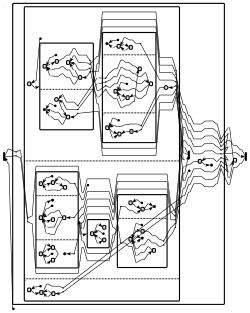
\includegraphics[scale=0.5]{Bilder/sample5.png}
    \caption{sample5}
    \label{fig:sample5}
\end{figure}
\begin{figure}[ht]
    \centering
    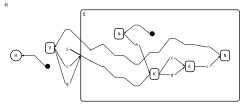
\includegraphics[scale=0.7]{Bilder/sample6.png}
    \caption{sample6}
    \label{fig:sample6}
\end{figure}